\section{Higher Order Linear Differential Equations}
The second order linear homogeneous equation \eqref{eq:2lde} is vital; it allows us to model a wide set of equations that are both found in nature, as well as purely theoretical.

    \begin{equation}\label{eq:2lde}
        m \ddot{x} + b \dot{x} + kx = f(t)
    \end{equation}\myequations{Second Order Linear Differential Equation}

    Where $x$ is our given equation, $\dot{x}$ is the first derivative of $x$, and $\ddot{x}$ is the second derivative of $x$. $f(t)$ is any equation. The behavior of this second order differential equation will vary based on the values of $m, b, k$, and $f(t)$.

    \subsection{Harmonic Oscillators}
    Our established equation for second order differential equations can help model many different types of behavior found in nature.

        \subsubsection{The Mass-Spring System}
        Consider an object with mass $m$ on a table that is attached to a spring attached to wall. When the object is moved by an external force, we can model its behavior using Newton's Second Law of Motion: $F = m \ddot{x}$ where $F$ is the sum of the forces acting on the object.

        \begin{figure}[h!]
            \centering
            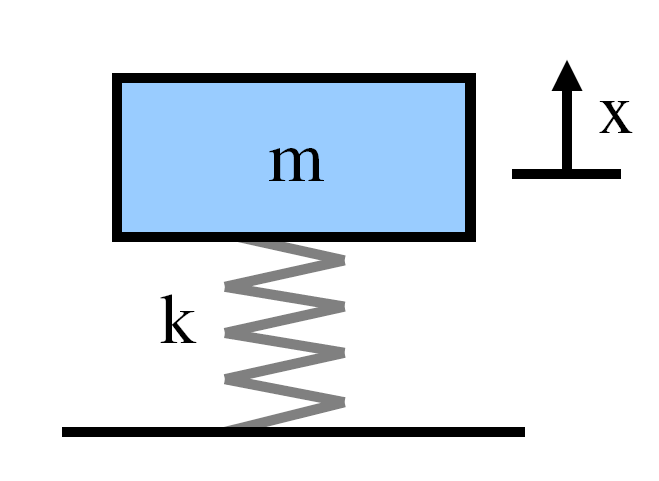
\includegraphics[scale=0.25]{./img/mass_spring.png}
            \label{fig:massspringsystem}
            \caption{Visual Representation of a Mass-Spring System}
        \end{figure}

        We have three different types of forces:

            \begin{itemize}
                \item \textbf{Restoring Force:} The restorative force of a spring is $\propto$ the amount of stretching/compression:
                    \[ F_{\text{restoring} } = -k x \]
                \item \textbf{Damping Force:} We also assume that friction exists, and therefore a damping force $\propto$ the velocity of the object:
                    \[ F_{\text{damping} } = -b \dot{x} \]
                    Where damping constant $b > 0$ and small for slick surfaces.
                \item \textbf{External Force:} We also allow for an external force to drive the motion:
                    \[ F_{\text{external} } = f(t) \]
            \end{itemize}

        Thus we get our equation for a Simple Harmonic Oscillator:

            \[ m \ddot{x} + b \dot{x} + kx = f(t) \]

            \begin{itemize}
                \item Constants $m>0, k>0, b>0$
                \item When $b=0$, the motion is called undamped. Otherwise it is damped.
                \item if $f(t)=0$, the equation is homogeneous and the motion is called unforced, undriven, or free. Otherwise it is forced, or driven.
            \end{itemize}

        \subsubsection{Solutions}
        When we say solution, we are referring to a solution that gives us $x$, in other words, the position of the mass at any given time $t$ as a function of $t$. Due to the inherent nature of derivatives, this may or may not have undetermined constants (often denoted as $[c_1, c_2, \dots, c_n]$) as will be set by initial values given (similar to first order differential equations).

        Later we will determine how to solve these equations fully, however a quick answer can be found by applying the following formulas. After learning the methods given ahead, be sure to come back and determine how these solutions were determined.

            \[ \begin{aligned}
                \text{Given Equation: } m \ddot{x} + kx = 0\\
                x(t) = c_1 \cos \left( \omega_0 t \right) + c_2 \sin \left( \omega_0 t \right)\\
                \omega_0 = \sqrt{\frac{k}{m} }
            \end{aligned} \]

        This gives us one form of the solution, however we can also find an alternate form:

            \[ x(t) = A \cos \left( \omega_0 t - \delta \right) \]

        Where
            \begin{itemize}
                \item Amplitude $A$ and phase angle $\delta$ (radians) are arbitrary constants determined by initial conditions.
                \item The motion has circular frequency $\omega_0 = \sqrt{\frac{k}{m} }$ (radians) per second, and a natural frequency $f_0 = \frac{\omega_0}{2 \pi}$
                \item The period $T$ (seconds) is $2 \pi \sqrt{\frac{m}{k} }$
                \item The above solution is a horizontal shift of $A \cos (\omega_0 t)$ with phase shift $\frac{\delta}{\omega_0}$.
            \end{itemize}

        To convert between the two forms, apply the following formulas.

            \[
                \begin{cases}
                    A = \sqrt{c_1^2 + c_2^2}\\
                    \tan \delta = \frac{c_2}{c_1}
                \end{cases}
                \begin{cases}
                    c_1 = A \cos \delta\\
                    c_2 = A \sin \delta
                \end{cases}
            \]

        To solve the Mass-Spring System with both damping and forcing as given by the following equation:

            \[
                m \ddot{x} + b\dot{x} + kx = F_0 \cos ( \omega_f t )
            \]

        we can apply the following formula. (Note, some concepts are explained later in the text, refer back if needed)

        \begin{enumerate}
            \item $x_h(t)$ has three possible solutions. See \eqref{sec:2deroots}.
            \item $x_p(t)$ can be assumed as
                \[ A \cos ( \omega_f t ) + B \sin ( \omega_f t )\]
                See \eqref{sec:2decoefficients}.
            \item \[ \omega_0 = \sqrt{\frac{k}{m} } \]
            \item \[ A = \frac{m (\omega_0^2 - \omega_f^2) F_0}{m^2{(\omega_0^2 - \omega_f^2)}^2 + {(b \omega_f)}^2} \]
            \item \[ B = \frac{b \omega_f F_0}{m^2{(\omega_0^2 - \omega_f^2)}^2 + {(b \omega_f)}^2} \]
        \end{enumerate}

        As you can see, this is a pain. Values $A$ and $B$ in particular are tedious to calculate. Despite this, as you'll see later, these methods can be easier than solving by hand.

        \subsubsection{Phase Planes}\label{sec:2depplane}
        For any autonomous second order differential equation

            \[ \ddot{x} = F(x, \dot{x}) \]

        the phase plane is the two dimensional graph with $x$ and $\dot{x}$ axes (which are the position and velocity respectively)\footnote{This concept of a phase plane is identical to the one introduced in \eqref{sec:visde} with the exception of $\dot{x}$ replacing $y$.}. This phase plane has a vector field with direction given by

            \[ \begin{cases}
                    H \to \frac{dx}{dt} = \dot{x}\\
                    V \to \frac{d\dot{x} }{dt} = \ddot{x}
                \end{cases} \]

        Trajectories can be formed by parametrically combining the vectors into a path. A graph showing these trajectories is called a phase portrait.

        The differential equation is also equivalent to the system of equations:

            \[ \begin{cases}
                    \dot{x} = y\\
                    \dot{y} = \ddot{x} = f(t) - \frac{k}{m} x - \frac{b}{m} y
                \end{cases} \]

        The biggest advantage with phase portraits is that is allows the user to solve the differential equation graphically, and not numerically. This can be much easier if done correctly.

    \subsection{Properties and Theorems}
    For the linear homogeneous, second-order differential equation

        \[
            y\prime\prime + p(t) y\prime + q(t)y = 0
        \]

    with $p$ and $q$ being continuous functions of $t$, there exists a two-dimensional vector space of solutions.

    Rewriting the above equation gives us

        \[
            y\prime\prime(t) \equiv f(t, y, y\prime) = -p(t) y\prime - q(t) y = 0
        \]

    which gives us the existence and uniqueness theorem for the second order equation.

        \begin{thm}[Existence and Uniqueness]\label{thm:2eau}
            Let $p(t)$ and $q(t)$ be continuous on $a, b$ containing $t_0$. For any $A$ and $B$ in $\mathbb{R}$, there exists a unique solution $y(t)$ defined on $(a, b)$ to the IVP
            \[
            y\prime\prime + p(t) y\prime + q(t)y = 0, y(t_0) = A, y\prime(t_0) = B
            \]
        \end{thm}

    A basis exists for the general second order equation.

        \begin{thm}[Solution Space]\label{thm:solutionspace}
            The solution space $S$ for a second order homogeneous differential equation has a Dimension of 2.
        \end{thm}

    For any linear second order homogeneous differential equation on $(a, b)$,

        \[
            y\prime\prime + p(t) y\prime + q(t)y = 0
        \]

    for which $p$ and $q$ are continuous on $(a, b)$, any two linearly independent solutions $\{y_1, y_2\}$ form a basis of the solutions space $S$, and every solution $y$ on $(a, b)$ can be written as

        \[
            y(t) = c_1 y_1(t) + c_2 y_2(t) \to (c_1, c_2) \in \mathbb{R}
        \]

    To generalize we can apply the same principle to $nth$ order differential equations.

        \begin{thm}[Existence and Uniqueness for $nth$ Order Differential Equations]\label{thm:neau}
        Let $p_1(t), p_2(t), \dots, p_n(t)$ be continuous functions on $(a, b)$ containing $t_0$. For any initial values $A_0, A_1, \dots, A_{n-1} \in \mathbb{R}$, there exists a unique solution $y(t)$ to the IVP
        \[
        \begin{aligned}
            y\prime\prime(tp_1(t)y^{n - 1}(t)) + p_1(t)y^{n - 1}(t) + p_2(t)y^{n - 2}(t) + \cdots + p_n(t)y(t) = 0\\
            y(t_0) = A_0, y\prime(t_0) = A_1, \dots, y^{n - 1}(t_0) = A_{n-1}
        \end{aligned}
        \]
    \end{thm}

    For $n$th order differential equations, our solution space theorem \eqref{thm:solutionspace} applies, just replace the term ``2'' and ``second'' with ``$n$'' and ``$n$th''.

    \subsection{Roots}\label{sec:2deroots}
    If given a second order equation in the form $a \ddot{y} + b \dot{y} + cy = 0$, we can use our previous definition of a first order differential equation to find an easier method of solving. At its core, this method consists of converting our given second order differential equation and converting it into a quadratic equation, using which we can solve for the homogeneous solution.

        \begin{equation}\label{eq:2de-quad}
            a \ddot{y} + b \dot{y} + cy = 0 \Leftrightarrow ar^2 + br + c = 0
        \end{equation}\myequations{Quadratic form of the Second Order Linear Differential Equation}

    The resulting equation is called the characteristic equation. Solutions to this equation are called characteristic roots. Due to the nature of quadratic equations, there are three different possibilities for the solution:

        \begin{itemize}
            \item Two distinct real roots or zeros
            \item One real root (a double root)
            \item Two imaginary roots
        \end{itemize}

    These are summarized as follows.

        \begin{table}[ht]
            \centering
            \begin{tabular}{| l | l | l |}
                \hline
                \textbf{Case One} & Real Unequal Roots & Overdamped Motion\\
                $\Delta > 0$ & $r_1, r_2 = \frac{-b \pm \sqrt{b^2 - 4ac} }{2a}$ & $y_h(t) = c_1 e^{r_1 t} + c_2 e^{r_2 t}$\\&&\\
                \hline
                \textbf{Case Two} & Real Repeated Root & Critically Damped Motion\\
                $\Delta = 0$ & $r = - \frac{b}{2a} $ & $y_h(t) = c_1 e^{r t} + c_2 t e^{r t}$\\&&\\
                \hline
                \textbf{Case Three} & Complex Conjugate Roots & Underdamped Motion\\
                $\Delta < 0$ & $r_1, r_2 = \alpha \pm \beta i$ & $y_h(t) = e^{\alpha t} \left( c_1 \cos \left(\beta t \right) + c_2 \sin \left( \beta t \right) \right)$\\
                & $\alpha = - \frac{b}{2a}, \beta = \frac{\sqrt{4ac - b^2} }{2a}$ &\\&&\\
                \hline
            \end{tabular}
            \caption{Roots for Second Order Differential Equations in Characteristic Equation Form}
            \label{table:roots}
        \end{table}

    These methods allow us to generalize for higher order differential equations and find solutions that would be otherwise impossible.

    \subsection{Linear Independence}
    The Solution Space Theorem \eqref{thm:solutionspace} provides us with the number of solutions in a bases for an $n$th order homogeneous differential equation ($n$).

    \begin{itemize}
        \item Starting with $m$ solutions for the $n$th order case, if $m > n$ the solutions can no be independent.
        \item If $m=n$, we must test using the concepts from before.
        \item If $m < n$, the set does not span the space.
    \end{itemize}

        \subsubsection{Wronskian}
        The Wronskian also tells us about the linear independence of a set of functions. This Wronskian is identical to the Wronskian previously defined \eqref{eq:wronskian}.

        Suppose $\{y_1, y_2, \dots, y_n \}$ is a set of solutions of an $n$th order homogeneous differential equation.

            \[
                L(y) = a_n(t)y^n + a_{n-1}(t)y^{n-1} + \cdots + a_1 (t)y\prime + a_0 (t)y = 0
            \]
            \begin{enumerate}
                \item If $W[y_1, y_2, \dots, y_n] \neq 0$ at any point on $(a, b)$, then the set is linearly independent.
                \item If $W[y_1, y_2, \dots, y_n] = 0$ at every point on $(a, b)$, then the set is linearly dependent.
            \end{enumerate}

    \subsection{Undetermined Coefficients}\label{sec:2decoefficients}
    Let's assume
        \[ L(y) = a_n(t)y^n + a_{n-1}(t)y^{n-1} + \cdots + a_1 (t)y\prime + a_0 (t)y = 0 \]
    where $t \in $ some interval $I$.

    If $y_i(t)$ is a solution of $L(y) = f_i(t)$, then
        \[ y(t) = c_1 y_1(t) = c_2 y_2(t) + \cdots + c_n y_n(t) \]
    is a solution of
        \[ L(y) = c_1 f_1(t) + c_2 f_2(t) + \cdots + c_n f_n(t) \]

    In order to apply this, we need the non-homogeneous principle.

    \begin{thm}[Non-Homogeneous Principle]
        \[
            y(t) = y_h(t) + y_p(t)
        \]
    \end{thm}

    What this basically boils down to is making educated guesses in order to identify the form of the particular solution, as well as eventually the particular solution itself. Once the particular and homogeneous solutions are identified, add them to determine the solution. The following table may help identify common formats and solution types.

    \begin{table}[ht]
        \centering
        \begin{tabular}{l | l | l}
            & $f(t)$ & $y_p(t)$\\
            \hline
            $\boxed{1}$ & $k$ & $A_0$\\
            $\boxed{2}$ & $P_n(t)$ & $A_0(t)$\\
            $\boxed{3}$ & $C e^{kt}$ & $A_0 e^{kt}$\\
            $\boxed{4}$ & $C \cos(\omega t) + D \sin(\omega t)$ & $A_0 \cos(\omega t) + B_0 \sin(\omega t)$ \\
            $\boxed{5}$ & $P_n(t) e ^{kt}$ & $A_n(t) e^{kt}$ \\
            $\boxed{6}$ & $P_n(t) \cos(\omega t) + Q_n(t) \sin(\omega t)$ & $A_n(t) \cos(\omega t) + B_n(t) \sin(\omega t)$ \\
            $\boxed{7}$ & $C e^{kt} \cos(\omega t) + D e^{kt} \sin(\omega t)$ & $A_0 e^{kt} \cos(\omega t) + B_0 e^{kt} \sin(\omega t)$ \\
            $\boxed{8}$ & $P_n(t) e^{kt} \cos(\omega t) + Q_n(t) e^{kt} \sin(\omega t)$ & $A_n(t) e^{kt} \cos(\omega t) + B_n(t) e^{kt} \sin(\omega t)$ \\
        \end{tabular}
        \caption{Guesses for Particular Solutions}
        \label{table:guessings}
    \end{table}

    \begin{itemize}
        \item $P_n(t), Q_n(t), A_n(t), B_n(t) \in \mathbb{P}$
        \item $A_0, B_0 \in \mathbb{P}_0 \equiv \mathbb{R}$
        \item $k, \omega, C, D \in \mathbb{R}$
        \item In $\boxed{4}$ and $\boxed{6}-\boxed{8}$ both terms must be in $y_p$ even if only one term is present in $f(t)$.
    \end{itemize}

    If any term or terms of $y_p$ is found in $y_h$, multiply the term by $t$ or $t^2$ to eliminate the duplication.

    \subsection{Variation of Parameters}
    We've already used variation of parameters to find the solutions of $y\prime + p(t) y = f(t)$. This same strategy can be applied to second order equations in the form:

        \[ y\prime\prime + p(t)y\prime + q(t)y = f(t) \]

    To apply this method, follow these steps.

        \begin{enumerate}
            \item Find two linearly independent solutions of the second order differential equation
                    \[ y\prime\prime + p(t)y\prime + q(t)y = f(t) \]
                this having the general solution
                \[ y_h(t) = c_1 y_1(t) + c_2y_2(t) \]
            \item To find the particular solution, take
                \[ y_h(t) = c_1 y_1(t) + c_2y_2(t) \]
                and swap constants to get
                \[ y_p(t) = v_1(t) y_1(t) + v_2(t)y_2(t) \]
                where $v_1$ and $v_2$ are unknown functions.
            \item We find $v_1$ and $v_2$ by substituting our new equation into our first. Differentiating by the product rule we get
                \[ y_p\prime(t) = v_1 y_1\prime + v_2y_2\prime + v_1\prime y_1 + v_2\prime y_2 \]
            \item Before we calculate $y_p\prime\prime$ we choose an auxiliary condition, that $v_1$ and $v_2$ satisfy
                \[ v_1\prime y_1 + v_2\prime y_2 = 0 \]
                where we get
                \[ y_p \prime = v_1 y_1\prime + y_2\prime v_2 \]
            \item Differentiating again we get
                \[ y_p\prime\prime(t) = v_1 y_1\prime\prime + v_2 y_2\prime\prime + v_1\prime y_1\prime + v_2\prime y_2\prime \]
            \item We wish to get
                \[ L(y) = y\prime\prime + py\prime + qy = f \]
                Substituting for what we have solved for gives
                \[ v1 y_1\prime + v_2\prime y_2\prime = 0 \]
            \item We now have two equations for our two unknowns.
                \[ \begin{cases}
                    y_1 v_1\prime + y_2 v_2\prime = 0\\
                    y_1\prime v_1\prime + y_2\prime v_2\prime = f
                 \end{cases} \]
            \item Solve the system of equations and insert.
        \end{enumerate}

    Another method is to use Cramer's Rule \eqref{eq:cramer} where

        \[
            v_1\prime = \frac{\abs{\left[ \begin{matrix}
                0 & y_2\\
                f & y_2\prime\\
            \end{matrix} \right]} }{\abs{\left[ \begin{matrix}
                y_1 & y_2\\
                y_1\prime & y_2\prime\\
            \end{matrix} \right]} }
            \text{ and }
            v_2\prime = \frac{\abs{\left[ \begin{matrix}
                y_1 & 0\\
                y_1\prime & f\\
            \end{matrix} \right]} }{\abs{\left[ \begin{matrix}
                y_1 & y_2\\
                y_1\prime & y_2\prime\\
            \end{matrix} \right]} }
        \]

    The denominator in this case is the Wronskian. It will not be zero because both $y_1$ and $y_2$ are linearly independent. Integrate these to find $v_1$ and $v_2$.

\section{Linear Transformations}
Vectors that aren't rotated by linear transformations, but are only scaled or flipped are called eigenvectors.

\begin{thm}[Eigenvalues and Eigenvectors]
    Let $T: \mathbb{V} \to \mathbb{V}$ be a linear transformation. A scalar $\lambda$ is an eigenvalue of $T$ is there is a nonzero vector $\vec{v} \in \mathbb{V}$ such that $T(\vec{v}) = \lambda \vec{v}$.

    Such a nonzero vector $\vec{v}$ is called an eigenvector of $T$ corresponding to $\lambda$.

    If the linear transformation $T$ is regenerated by an $n\times n$ matrix $A$ where $\mathbb{V} = \mathbb{R}^n$ and $T(\vec{v}) = A \vec{v}$, then $A$ and $\vec{v}$ are characterized by the equation $A \vec{v} = \lambda \vec{v}$.
\end{thm}

To compute these eigenvalues and eigenvectors, follow the following steps\footnote{Note, the same exact steps are followed even if we have $\lambda$ to be in terms of $i$. The only exception is that we are no longer in any $\mathbb{R}^n$ space, and therefore there will be no \textit{real} eigenspace (See \eqref{sec:eigenspaces})}.

\begin{enumerate}
    \item Write the characteristic equation
        \[ \lvert A - \lambda I \rvert = 0 \]
    \item Solve the characteristic equation for the eigenvalues.
    \item For each eigenvalue, find the eigenvector by solving
        \[ \left( A - \lambda_i I \right) \vec{v}_i = 0 \]
\end{enumerate}

As you'd imagine, once the size of a matrix becomes larger than 2 or 3, these steps are tedious and long. Computers to the rescue!

    \subsection{Example}
    Find the eigenvalues and eigenvectors of

        \[ \ma =
            \left[ \begin{array}{rrr}
                1 & 1 & -2\\
                -1 & 2 & 1\\
                0 & 1 & -1
            \end{array} \right] \]

        \begin{enumerate}
            \item Form the characteristic equation
                \[
                    \lvert \ma - \lambda \mathbf{I} \rvert = 
                    \left| \begin{array}{rrr}
                        1 - \lambda & 1 & -2\\
                        -1 & 2 - \lambda & 1\\
                        0 & 1 & -1 - \lambda
                    \end{array} \right|  = 0 \]
            \item Simplifying we get
                \[ \lambda^3 - 2 \lambda^2 - \lambda + 2 = 0 \]
                We simplify and obtain
                \[ (\lambda - 2)(\lambda - 1)(\lambda + 1) = 0 \]
                Giving us roots of
                \[ \boxed{\lambda = \begin{cases}
                    2\\
                    1\\
                    -1
                \end{cases} } \]
            \item For each eigenvalue we solve $( \ma - \lambda_i \mathbf{I}) \vec{v}_i = \vec{0}$ for the associated eigenvector.
                \begin{itemize}
                    \item For $\lambda_1 = 2$ we obtain
                        \[
                            \left[ \begin{array}{rrr}
                                -1 & 1 & -2\\
                                -1 & 0 & 1\\
                                0 & 1 & -3
                            \end{array} \right]
                            \left[ \begin{array}{r}
                                v_1\\ v_2\\ v_3
                            \end{array} \right]
                            = \vec{0}
                        \]
                        With RREF
                        \[
                            \left[ \begin{array}{rrr|r}
                                1 & 0 & -1 & 0\\
                                0 & 1 & -3 & 0\\
                                0 & 0 & 0 & 0
                            \end{array} \right]
                        \]
                        Therefore $v_1 = v_3$, and $v_2 = 3 v_3$ giving us an answer of
                        \[
                            \boxed{
                                \vec{v}_1 =
                                \left[ \begin{array}{r}
                                    1\\ 3\\ 1
                                \end{array} \right]
                                \to \lambda_1 = 2
                            }
                        \]
                    \item For $\lambda_2 = 1$ we obtain
                        \[
                            \left[ \begin{array}{rrr}
                                0 & 1 & -2\\
                                -1 & 1 & 1\\
                                0 & 1 & -2
                            \end{array} \right]
                            \left[ \begin{array}{r}
                                v_1\\ v_2\\ v_3
                            \end{array} \right]
                            = \vec{0}
                        \]
                        With RREF
                        \[
                            \left[ \begin{array}{rrr|r}
                                1 & 0 & -3 & 0\\
                                0 & 1 & -2 & 0\\
                                0 & 0 & 0 & 0
                            \end{array} \right]
                        \]
                        Therefore $v_1 = 3v_3$, and $v_2 = 2 v_3$ giving us an answer of
                        \[
                            \boxed{
                                \vec{v}_1 =
                                \left[ \begin{array}{r}
                                    3\\ 2\\ 1
                                \end{array} \right]
                                \to \lambda_2 = 1
                            }
                        \]
                    \item For $\lambda_3 = -1$ we obtain
                        \[
                            \left[ \begin{array}{rrr}
                                2 & 1 & -2\\
                                -1 & 3 & 1\\
                                0 & 1 & 0
                            \end{array} \right]
                            \left[ \begin{array}{r}
                                v_1\\ v_2\\ v_3
                            \end{array} \right]
                            = \vec{0}
                        \]
                        With RREF
                        \[
                            \left[ \begin{array}{rrr|r}
                                1 & 0 & -1 & 0\\
                                0 & 1 & 0 & 0\\
                                0 & 0 & 0 & 0
                            \end{array} \right]
                        \]
                        Therefore $v_1 = v_3$, and $v_2 = 0$ giving us an answer of
                        \[
                            \boxed{
                                \vec{v}_1 =
                                \left[ \begin{array}{r}
                                    1\\ 0\\ 1
                                \end{array} \right]
                                \to \lambda_3 = -1
                            }
                        \]
                \end{itemize}
        \end{enumerate}

    \subsection{Special Cases}
    Some special cases to watch out for:
        \begin{itemize}
            \item \textbf{Triangular Matrices:} The eigenvalues of a triangular matrix (upper \textit{or} lower) appear on the main diagonal.
            \item \textbf{$2 \times 2$ Matrices:} The eigenvalues can be determined with
                \[ \lambda^2 - (Tr\footnote{Where $Tr(\ma)$ is the Trace of a matrix, i.e. the sum of the main diagonal.}(\ma)) \lambda + \lvert \ma \rvert = 0 \]
            \item \textbf{$3 \times 3$ Matrices:} Similarly:
                \[
                    \lambda^3 - \lambda^2 {\rm Tr}(\ma) - \lambda \frac{1}{2}\left( {\rm Tr}(\ma^2) - {\rm Tr}^2(\ma) \right) - \det(\ma) = 0
                \]
        \end{itemize}

    \subsection{Eigenspaces}\label{sec:eigenspaces}
    The set of all eigenvectors belonging to an eigenvalues $\lambda$ together with the zero vector form a subspace of $\mathbb{R}^n$ called the eigenspace.

        \begin{thm}[Eigenspaces]
            For each eigenvalue $\lambda$ of a linear transformation $T: \mathbb{V} \to \mathbb{V}$, the eigenspace
            \[
                \mathbb{E}_{\lambda} = \{ \vec{V} \in \mathbb{V} \, | \, T(\vec{v}) = \lambda \vec{v} \}
            \]
            is a subspace of $\mathbb{V}$.
        \end{thm}

        \begin{thm}[Distinct Eigenvalue]
            Let $\ma$ be an $n \times n$ matrix. If $\lambda_1, \lambda_2, \dots, \lambda_p$ are distinct eigenvalues with corresponding eigenvectors $\vec{v}_1, \vec{v}_2, \dots, \vec{v}_n$, then $\{\vec{v}_1, \vec{v}_2, \dots, \vec{v}_n\}$ is a set of linearly independent vectors.
            In other words, if each eigenvalue has one associated eigenvector, than that set of eigenvectors is linearly independent.
        \end{thm}

    \subsection{Properties of Eigenvalues}
    Let $\ma$ be an $n \times n$ matrix.

        \begin{itemize}
            \item $\lambda$ is an eigenvalue of $A$ if and only if
                \[ | \ma - \lambda \mathbf{I} | = 0 \]
            \item $\lambda$ is an eigenvalue of $A$ if and only if
                \[ ( \ma - \lambda \mathbf{I}) \vec{v} = \vec{0} \]
                has a non-trivial solution.
            \item $\ma$ has a zero eigenvalue if and only if
                \[ | \ma | = 0 \]
            \item $\ma$ and $\ma^T$ have the same characteristic polynomials and eigenvalues.
        \end{itemize}

    \subsection{The Mind-Blowing Part}
    Remember Characteristic Roots \eqref{sec:2deroots}? Well, they are \textit{identical} to eigenvalues as is evidenced below.

     Given the linear second order differential equation:

        \[ y\prime\prime - y \prime - 2y = 0 \]

    we know that it has a characteristic equation of

        \[ r^2 - r - 2 = (r - 2)(r + 1) = 0 \]

    with roots of

        \[
            [r_1, r_2]
            \begin{cases}
                2\\
                -1
            \end{cases}
        \]

    which creates the general solution of

        \[ y = c_1 e^{2t} + c_2 e^{-t} \]

    In Section \ref{sec:2depplane} we saw that we can write a second order differential equation as a system of equations:

        \[ \begin{cases}
            \dot{x} = y\prime\\
            \dot{y} = 2y + y\prime
        \end{cases} \]

        which has the matrix form $\vec{x}\prime = \ma \vec{x}$:

        \[ \vec{x} = \left[ \begin{array}{r}
            y\\
            y\prime
        \end{array} \right] \text{ and }
        \ma = \left[ \begin{array}{rr}
            0 & 1\\
            2 & 1
        \end{array} \right] \]

    The characteristic equation $| \ma - \lambda \mathbf{I} | = 0$ for this matrix $\ma$ is $\lambda^2 - \lambda - 2 = 0$ which has the same eigenvalues as our original equation has characteristic roots.

        \subsubsection{Properties of Linear Homogeneous Differential Equations with Distinct Eigenvalues}
        For the differential equation $\vec{x}\prime = \ma\vec{x}$ with distinct eigenvalues, the following properties apply.
            \begin{itemize}
                \item The domain of the linear transformation is a vector space of vector functions.
                \item The solution set is also a vector space of vector functions.
                \item The eigenspace for each eigenvalue is a one dimensional line in the direction of a vector in $\mathbf{R}^n$.
            \end{itemize}

